\chapter{Électronique}
\section{La lumière : Shield LDR}
\subsection{Schéma du Shield LDR}
\begin{figure}[h]
	\centering
	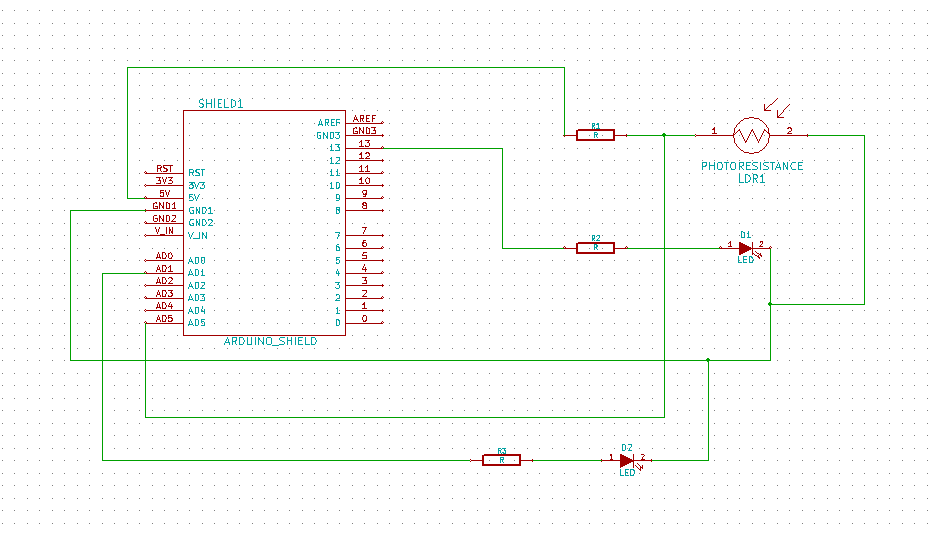
\includegraphics[width=550px]{images/SchemaElectriqueShield.png}
	\caption{Logiciel utilisé : Eeschema de Kicad}
\end{figure}

\subsection{Choix des composants} 
	Notre projet étant une reprise d'un projet de l'année dernière, nous avons du refaire le shield. On à donc récupéré leurs composants à savoir :
	\begin{itemize}
		\item Une Arduino Mega 2560
		\item Deux LEDs 
		\item Une photorésistance LDR
		\item Trois résistances
	\end{itemize}

\section{Alimentation autonome : 7805}
\subsection{Schéma du régulateur de tension}
\begin{figure}[h]
	\centering
	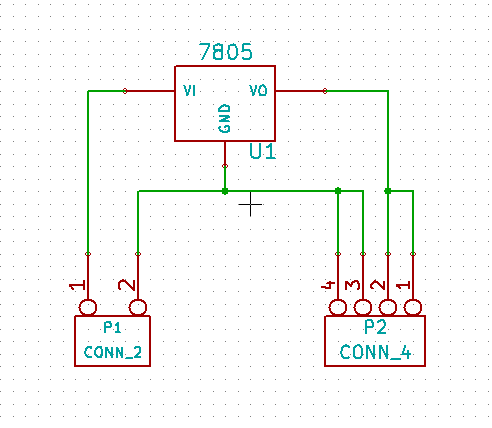
\includegraphics[width=350px]{images/SchemaDuRegulateur.png}
	\caption{Logiciel utilisé : Eeschema de Kicad}
\end{figure}

\subsection{Choix des composants} 
	Nos camarades de l'année dernière alimentaient leurs Arduino et Raspberry avec une prise secteur. Cette année, on a décidé d'en faire un réveil portable. Et qui dit portable, dit alimentation autonome. Les deux appareils étant alimentés en 5V, on a commandé un régulateur de tension 7805 qui délivre du 5V/1A. On met donc en entré du régulateur un pack d'accus de 7V et le régulateur va se charger de délivrer du 5V à l'arduino et à la raspberry branchées en dérivation sur celui-ci.

\section{Communication Arduino-Raspberry}
%Thibaud